\chapter{Análisis Exploratorio de los Datasets}
\label{app:anexo_eda}

Este apéndice recoge el análisis exploratorio de datos (EDA) realizado sobre el corpus combinado NeuroVoz + PC-GITA antes de la fase de modelado. El objetivo es caracterizar la distribución demográfica de los individuos, cuantificar el poder discriminativo de los biomarcadores acústicos mediante pruebas estadísticas no paramétricas, e ilustrar visualmente las diferencias entre pacientes con Enfermedad de Parkinson (EP) y sujetos de control sano (HC). Todos los análisis descritos en este apéndice se calcularon sobre el \textit{split} de entrenamiento (165 pacientes, 2.713 grabaciones) para evitar la fuga de información del conjunto de prueba.

% ===========================================================================
\section{Caracterización Demográfica de los Corpus}
% ===========================================================================

\subsection{Distribución de pacientes, sexo y edad}

El corpus combinado está compuesto por 207 pacientes, distribuidos de forma equilibrada entre los dos grupos diagnósticos (104 HC, 103 EP) y entre los dos conjuntos de datos (107 de NeuroVoz, 100 de PC-GITA). La \autoref{fig:eda_demo} presenta la caracterización demográfica completa: número de pacientes por corpus y grupo, proporción por sexo y distribución de edades.

\begin{figure}[htbp]
    \centering
    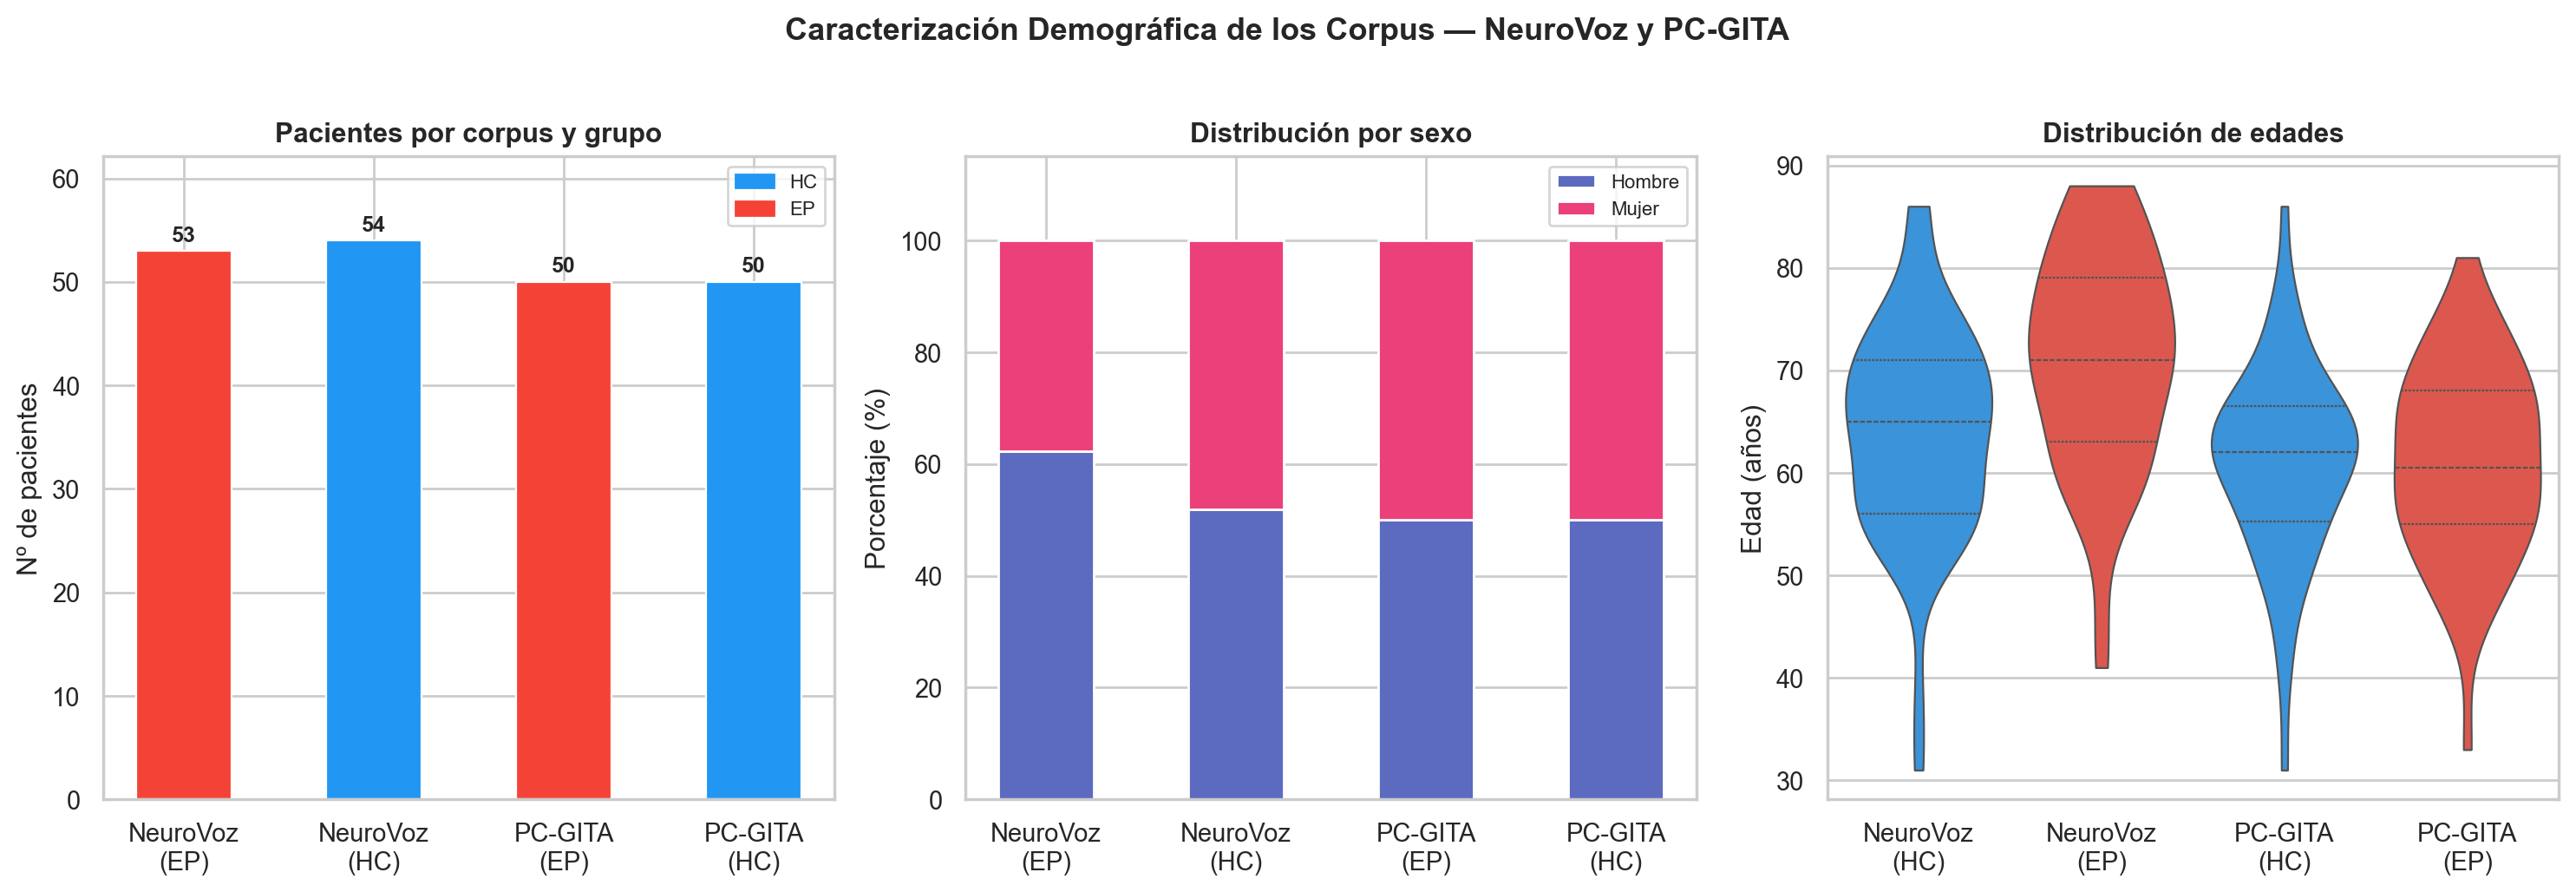
\includegraphics[width=\textwidth]{imagenes/eda/eda_01_demographics.png}
    \caption{Caracterización demográfica de los corpus. De izquierda a derecha: (a) número de pacientes por corpus y grupo diagnóstico; (b) distribución porcentual por sexo; (c) distribución de edades (diagramas de violín con cuartiles internos).}
    \label{fig:eda_demo}
\end{figure}

Se observan dos patrones relevantes. En primer lugar, ambos corpus presentan un ligero predominio masculino, especialmente en el grupo EP de PC-GITA (~70\,\% hombres), lo que refleja la mayor prevalencia de la Enfermedad de Parkinson en varones descrita en la literatura \cite{pringsheim2014}. En segundo lugar, el análisis de las distribuciones de edad revela una diferencia demográfica crítica entre los corpus:

\begin{itemize}
    \item \textbf{NeuroVoz:} el grupo EP presenta una edad media de $71.1 \pm 10.7$ años frente a $64.0 \pm 10.4$ años del grupo HC, lo que supone una diferencia de aproximadamente 7 años. Los grupos \textbf{no están emparejados por edad}, lo que introduce un potencial factor de confusión demográfico: cualquier modelo que incorpore la edad como variable predictora aprenderá, en parte, a predecir la demografía del locutor en lugar del diagnóstico clínico.
    \item \textbf{PC-GITA:} ambos grupos presentan una edad media de $61 \pm 9.4$ y $61 \pm 9.5$ años respectivamente. El corpus está \textbf{perfectamente emparejado por edad} (\textit{age-matched}), lo que lo convierte en el referente metodológico más riguroso para evaluar biomarcadores acústicos independientes del envejecimiento.
\end{itemize}

Esta asimetría motivó la evaluación de modelos con y sin la variable \texttt{Age} como predictor, reportándose los modelos \texttt{sin\_age} (solo características acústicas) como resultados principales por su mayor validez clínica.

\subsection{Distribución de grabaciones por actividad de habla}

La \autoref{fig:eda_recordings} muestra la distribución de grabaciones por actividad y grupo diagnóstico en cada corpus.

\begin{figure}[htbp]
    \centering
    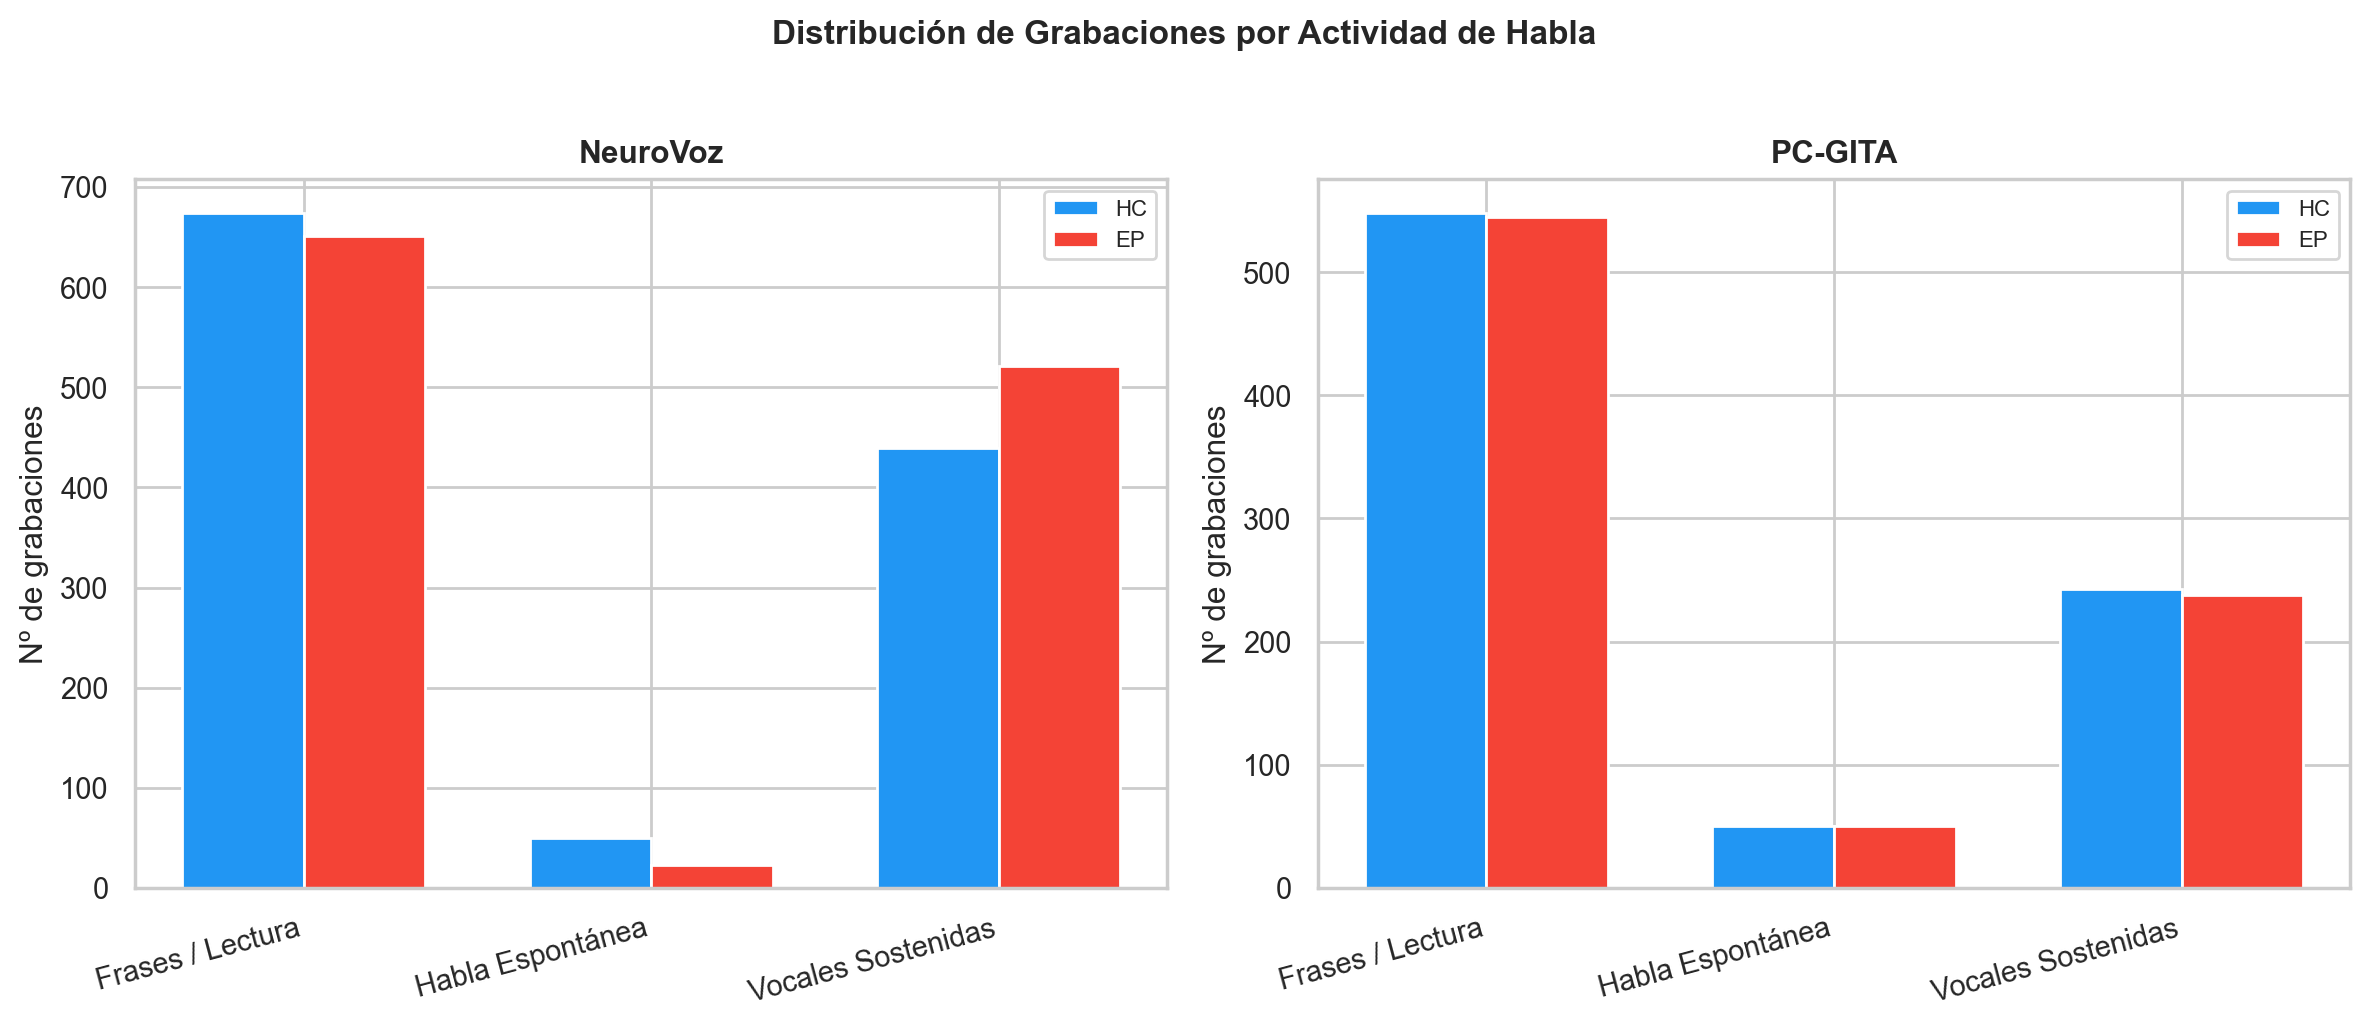
\includegraphics[width=\textwidth]{imagenes/eda/eda_02_recordings.png}
    \caption{Distribución de grabaciones por actividad de habla y grupo diagnóstico en NeuroVoz (izquierda) y PC-GITA (derecha).}
    \label{fig:eda_recordings}
\end{figure}

La actividad de \textbf{Frases / Lectura} es la más abundante en ambos corpus (~1.325 grabaciones en NeuroVoz, ~1.093 en PC-GITA), aportando la mayor potencia estadística para la detección. Las \textbf{Vocales Sostenidas} ocupan el segundo lugar (~960 y ~481 grabaciones respectivamente). El \textbf{Habla Espontánea} es la actividad más escasa y presenta un desequilibrio notable en NeuroVoz: 50 grabaciones HC frente a únicamente 23 EP, situación derivada de diferencias en el protocolo de grabación original del corpus. Este desbalance limita la potencia estadística de los análisis basados en habla espontánea de NeuroVoz y debe considerarse al interpretar los resultados obtenidos con esta modalidad.

% ===========================================================================
\section{Análisis Estadístico de los Biomarcadores Acústicos}
\label{sec:eda_biomarkers}
% ===========================================================================

\subsection{Diagramas de violín por corpus y actividad}

Las Figuras~\ref{fig:violin_nv_vocal}--\ref{fig:violin_pg_esp} muestran las distribuciones de los 16 biomarcadores para los grupos HC (azul) y EP (rojo) en cada una de las seis combinaciones corpus × actividad.

\begin{figure}[p]
    \centering
    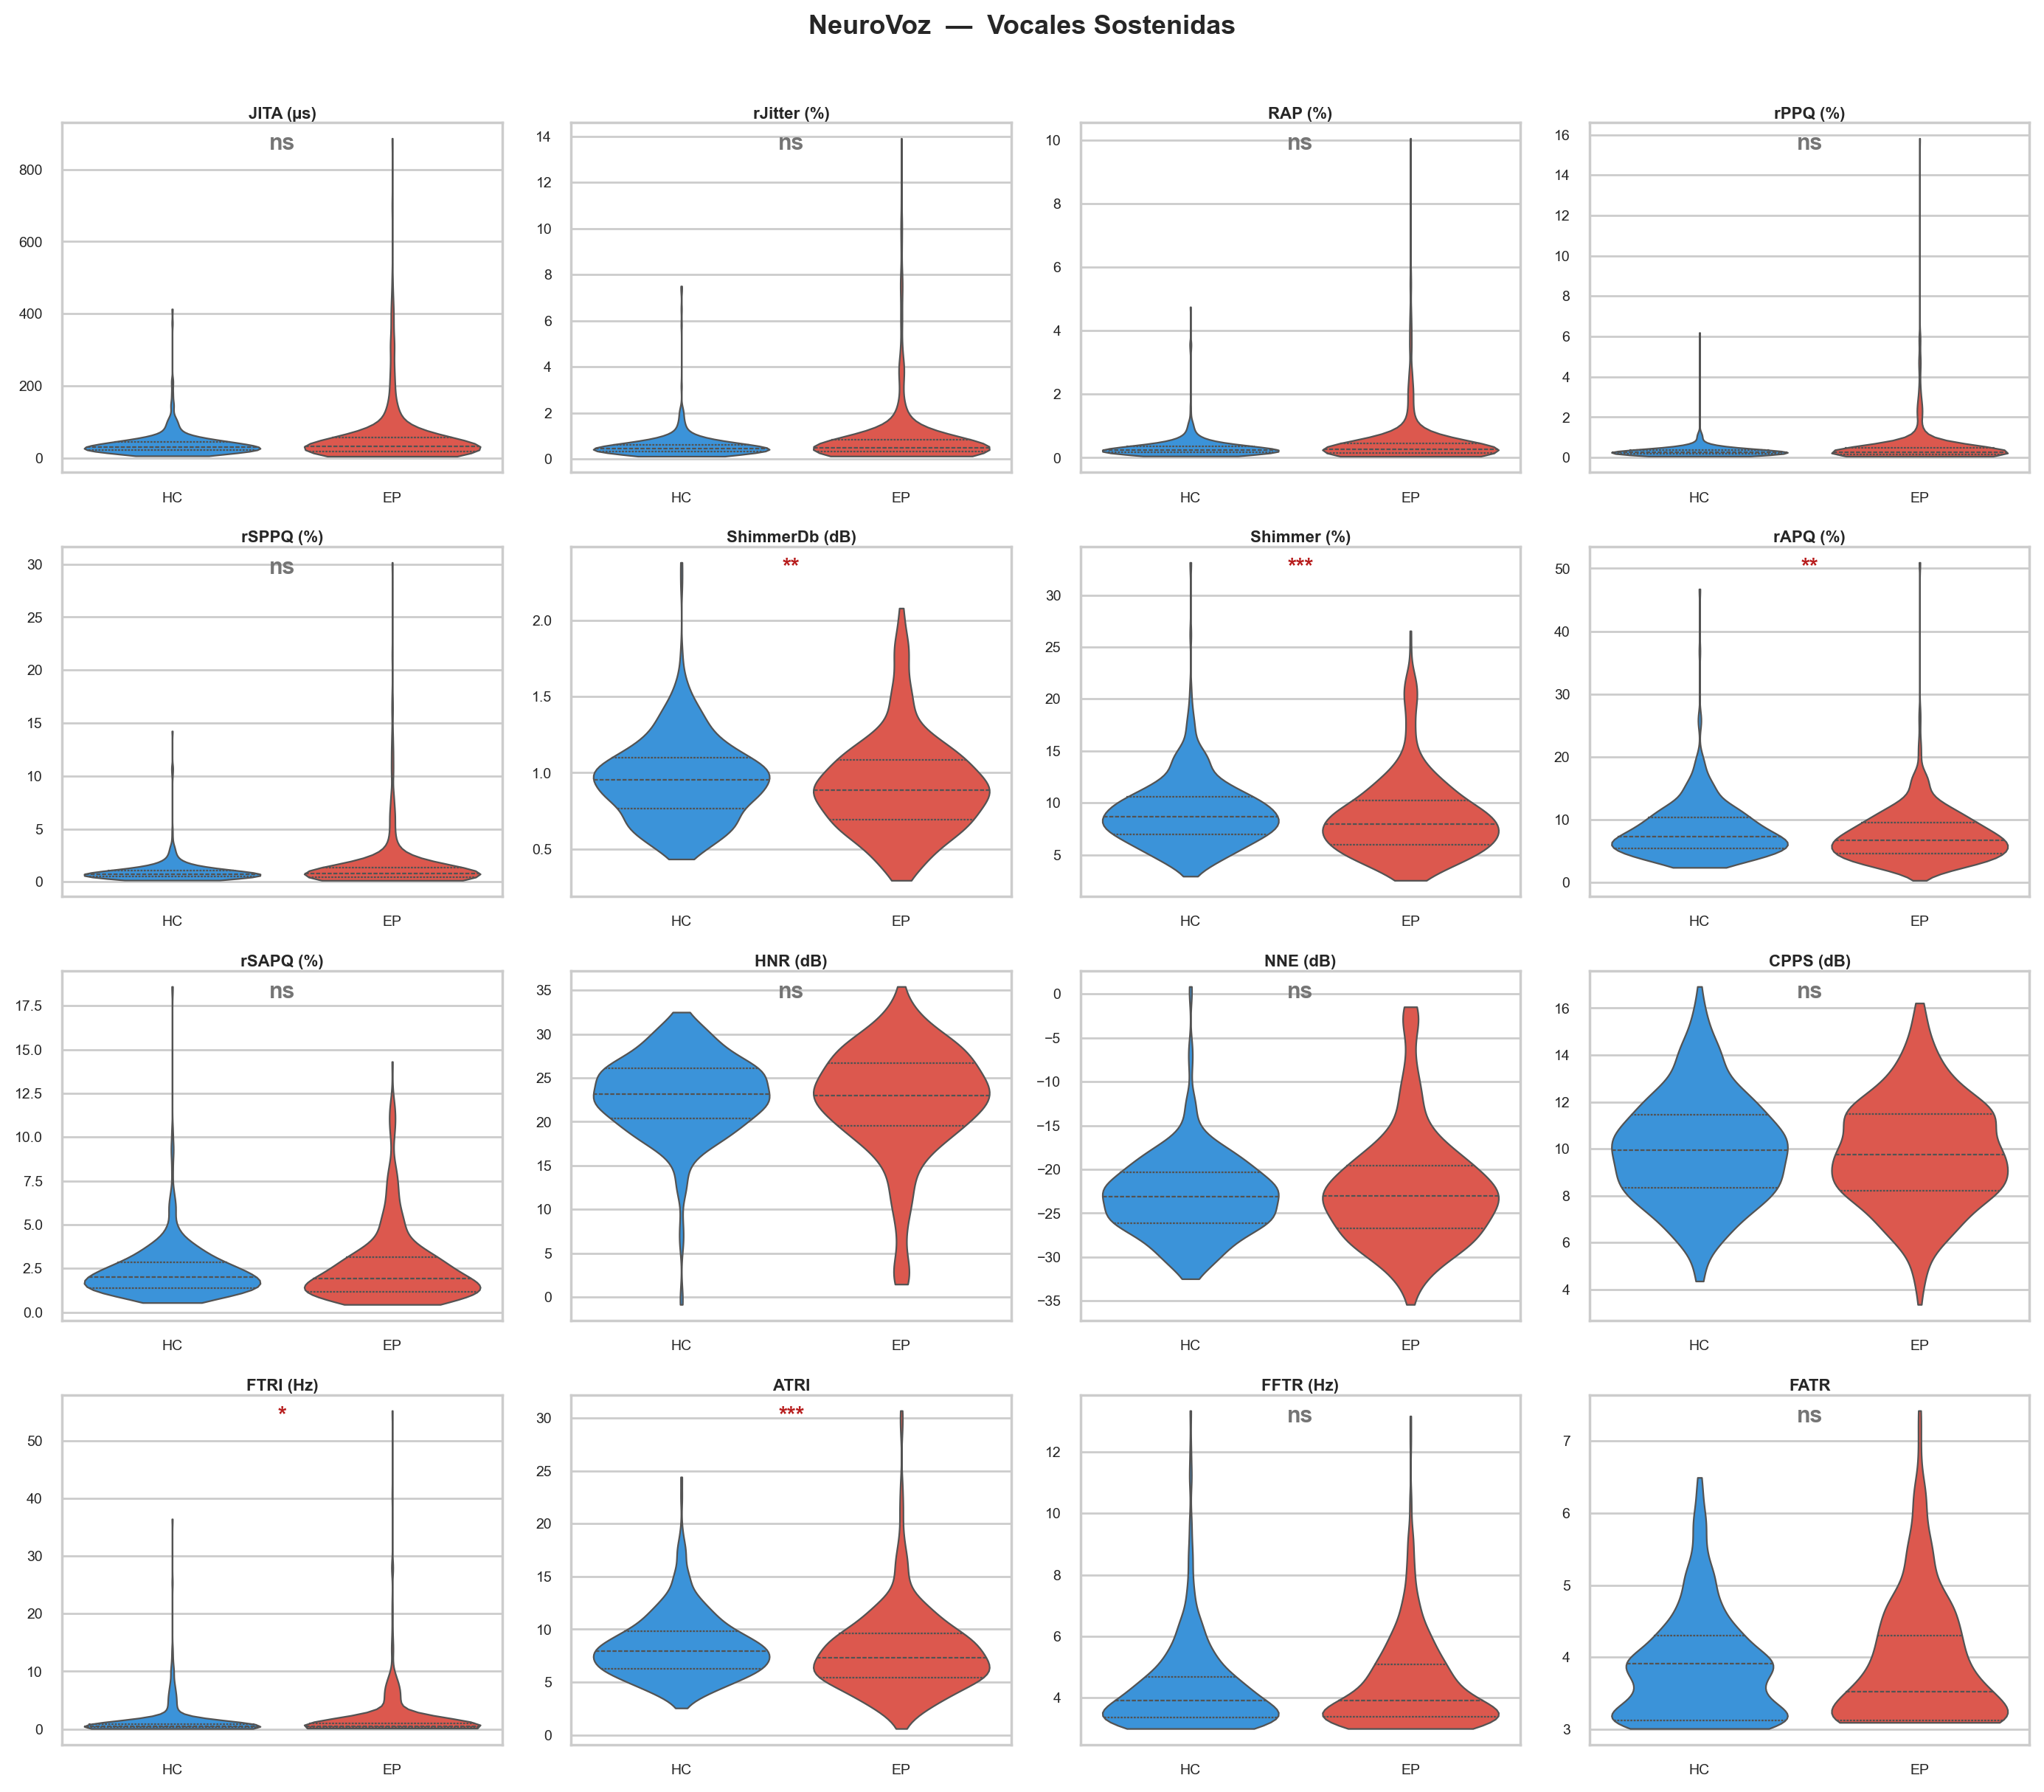
\includegraphics[width=\textwidth, height=0.88\textheight, keepaspectratio]{imagenes/eda/eda_violins_NV_vocal.png}
    \caption{Diagramas de violín — NeuroVoz, Vocales Sostenidas. Las líneas interiores marcan la mediana y los cuartiles Q1/Q3.}
    \label{fig:violin_nv_vocal}
\end{figure}

\begin{figure}[p]
    \centering
    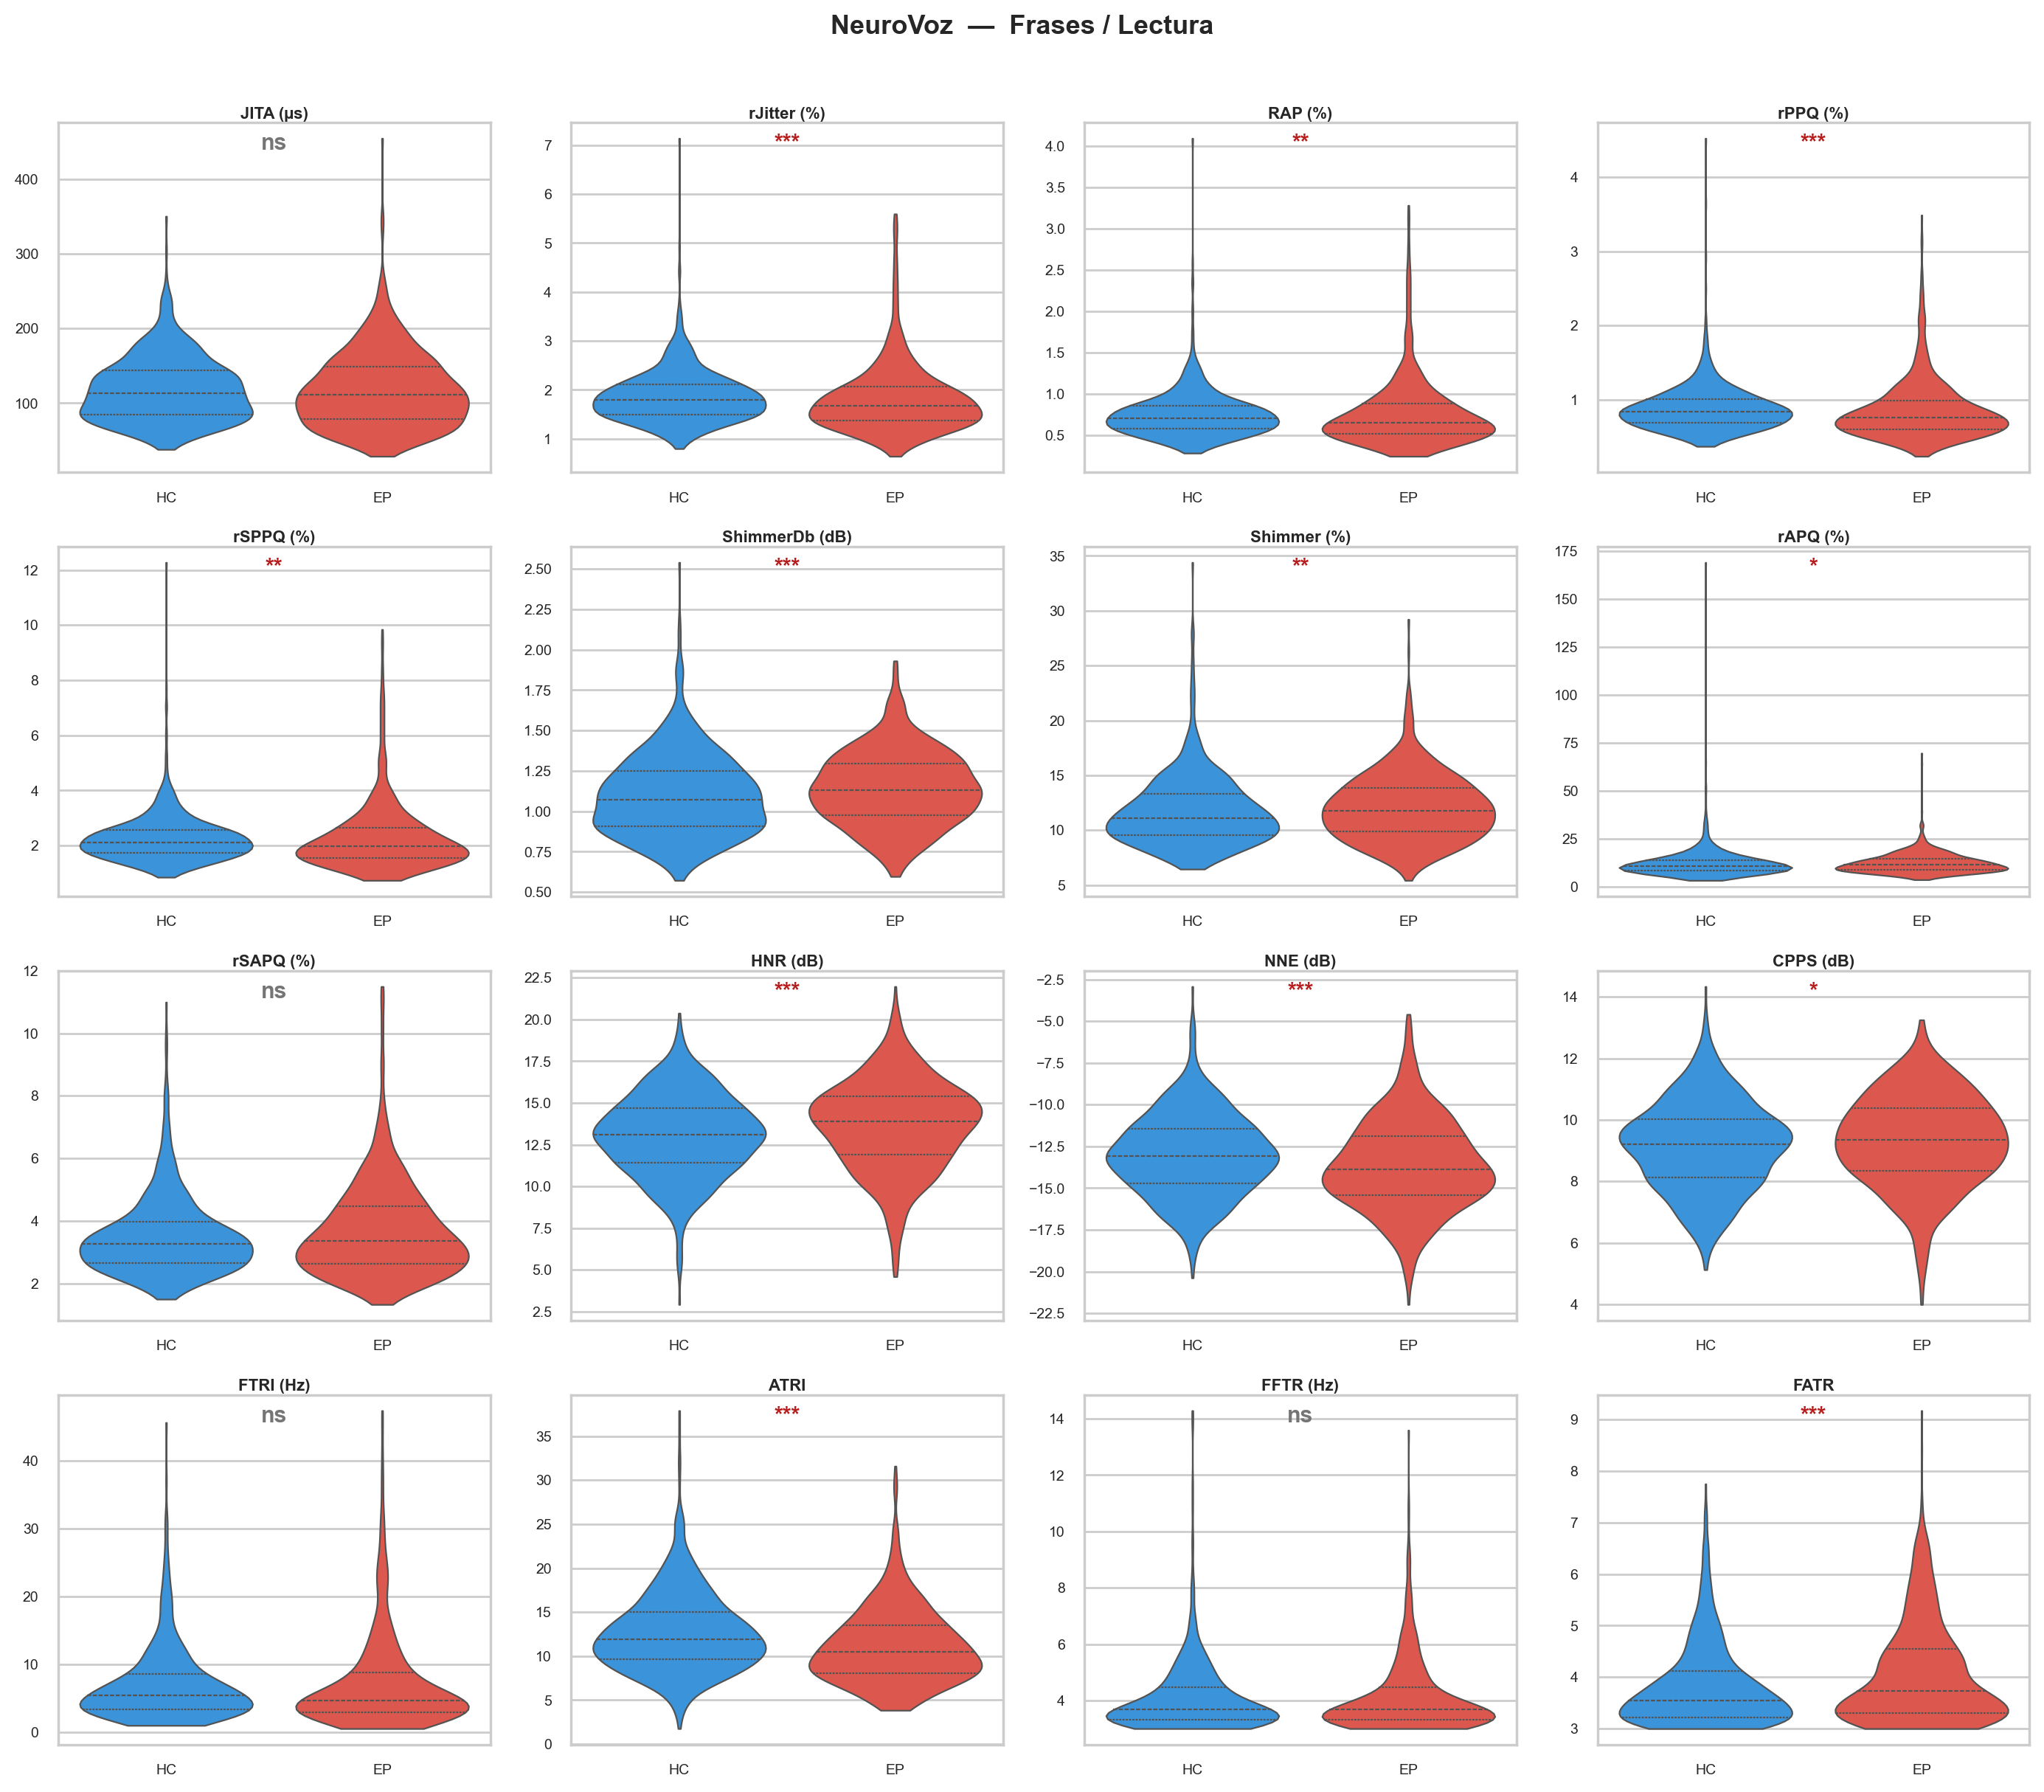
\includegraphics[width=\textwidth, height=0.88\textheight, keepaspectratio]{imagenes/eda/eda_violins_NV_frase.png}
    \caption{Diagramas de violín — NeuroVoz, Frases / Lectura.}
    \label{fig:violin_nv_frase}
\end{figure}

\begin{figure}[p]
    \centering
    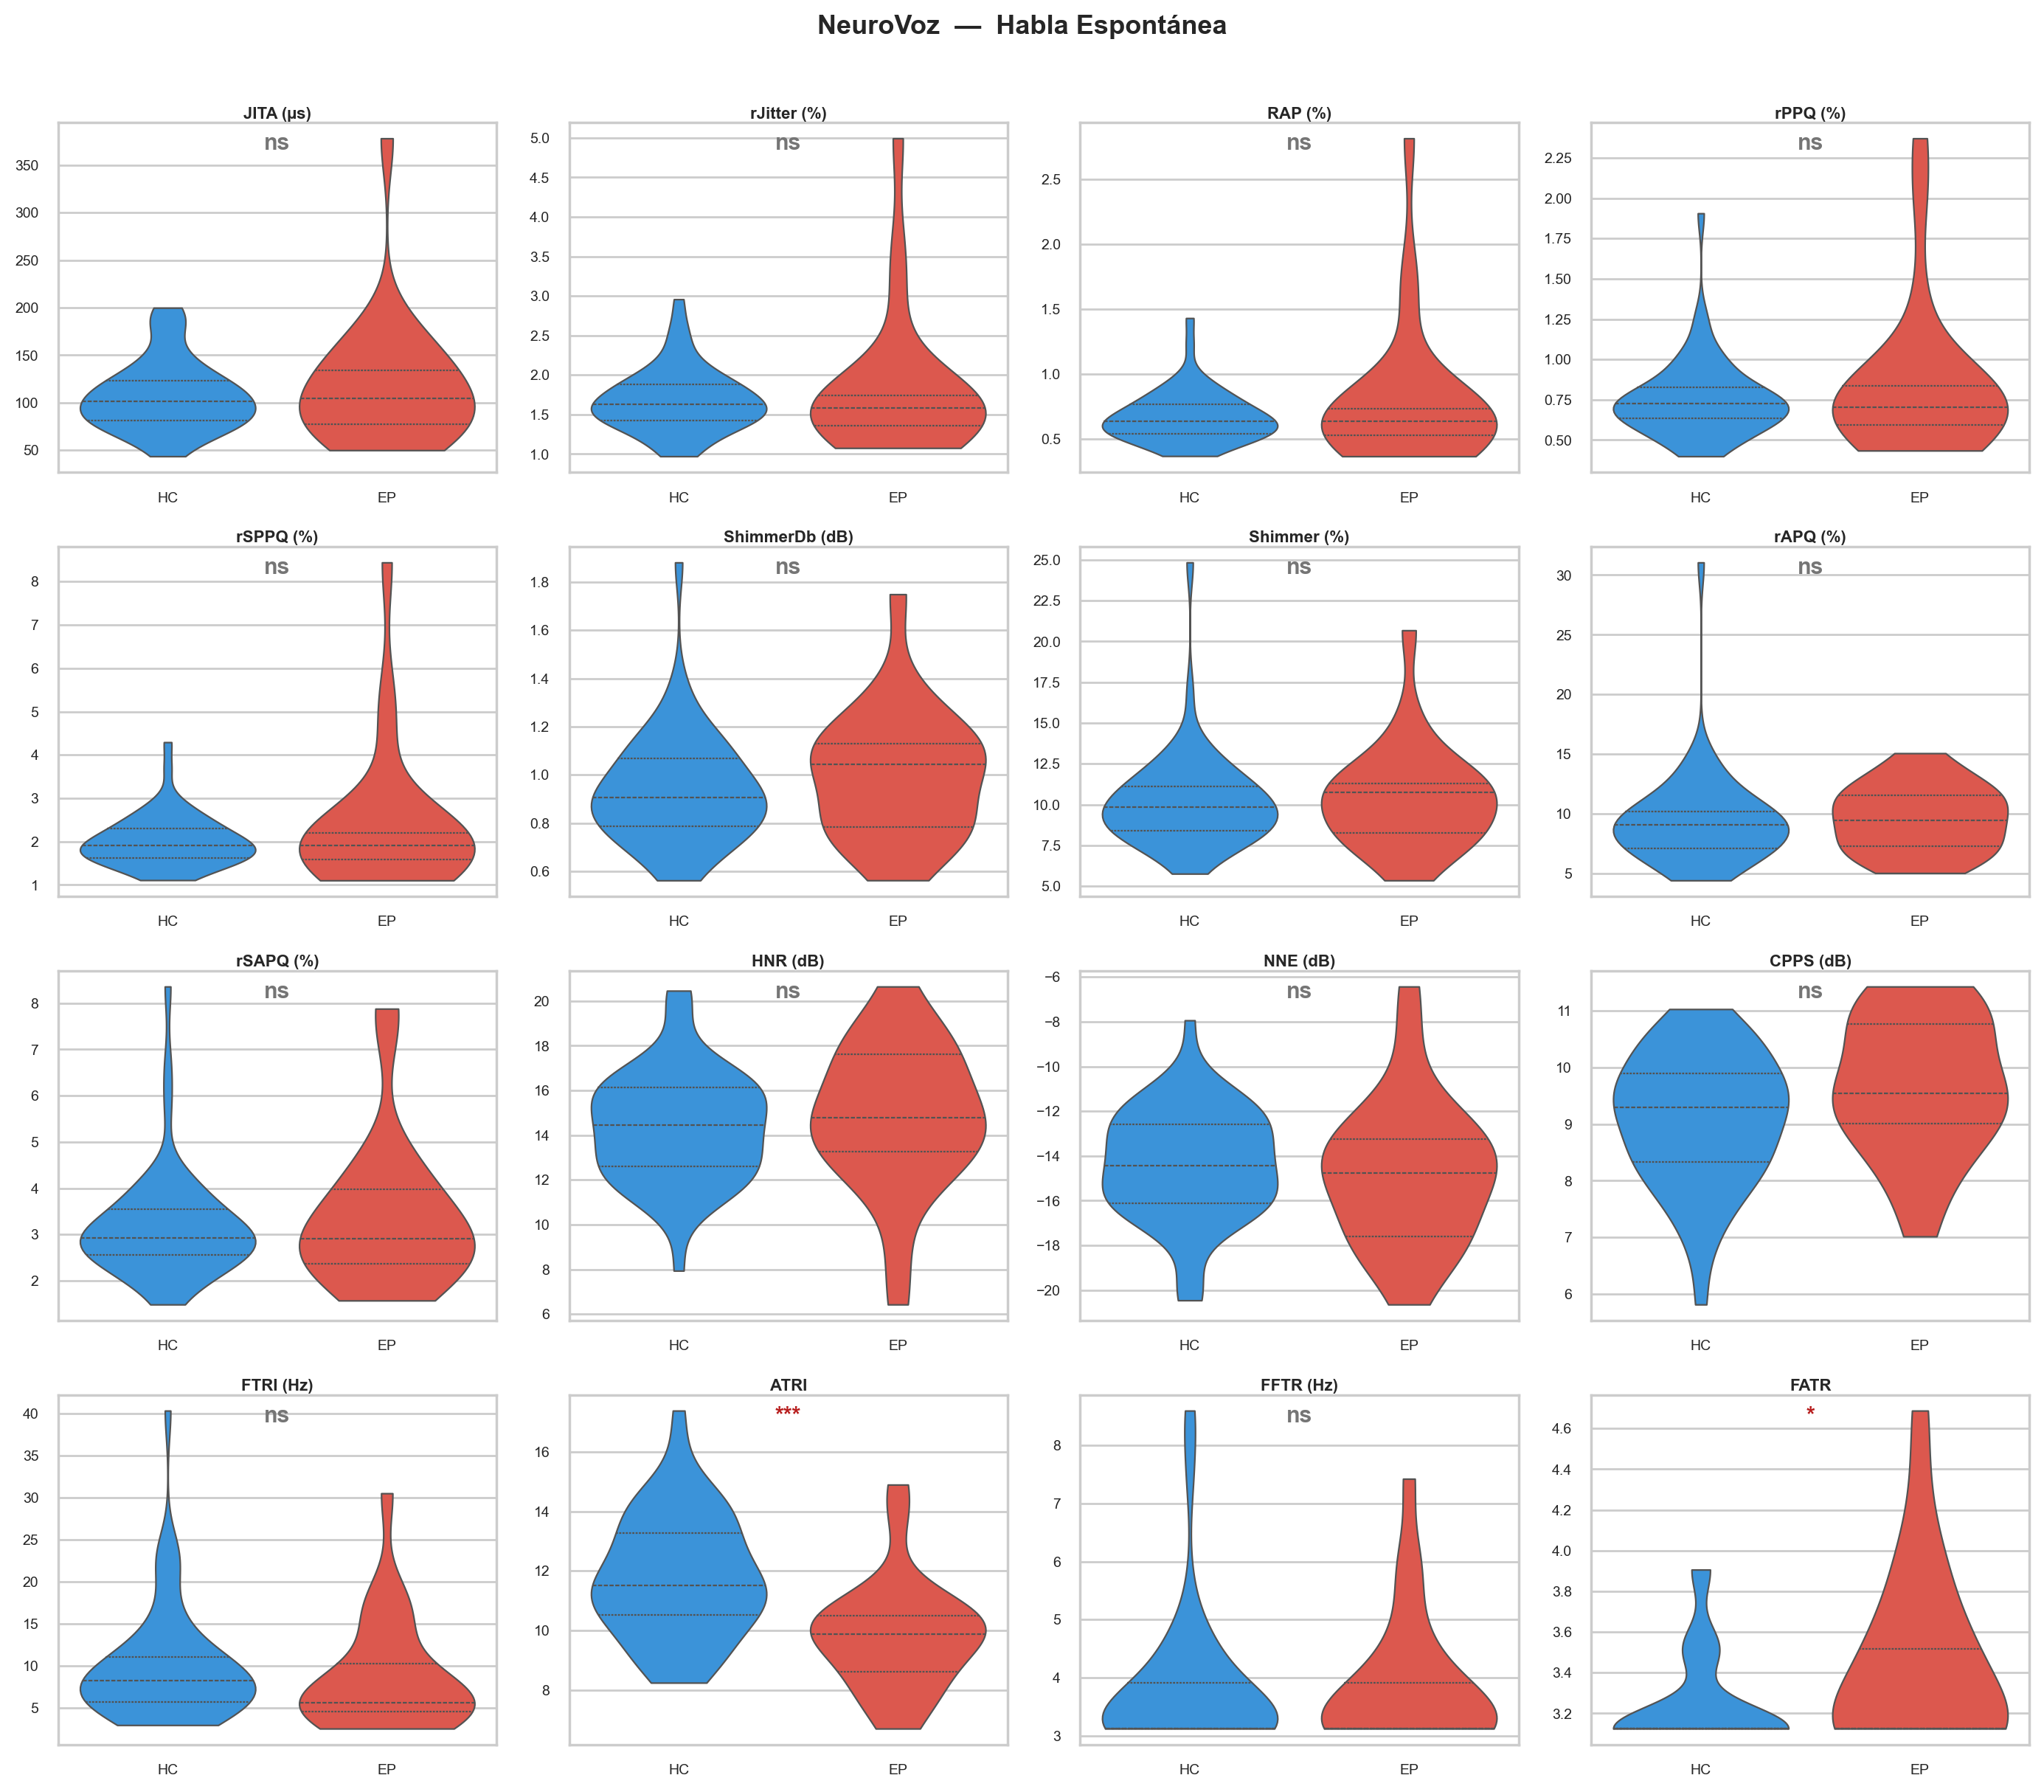
\includegraphics[width=\textwidth, height=0.88\textheight, keepaspectratio]{imagenes/eda/eda_violins_NV_espontanea.png}
    \caption{Diagramas de violín — NeuroVoz, Habla Espontánea. La mayoría de biomarcadores resulta no significativo por el reducido N del grupo EP (23 grabaciones).}
    \label{fig:violin_nv_esp}
\end{figure}

\begin{figure}[p]
    \centering
    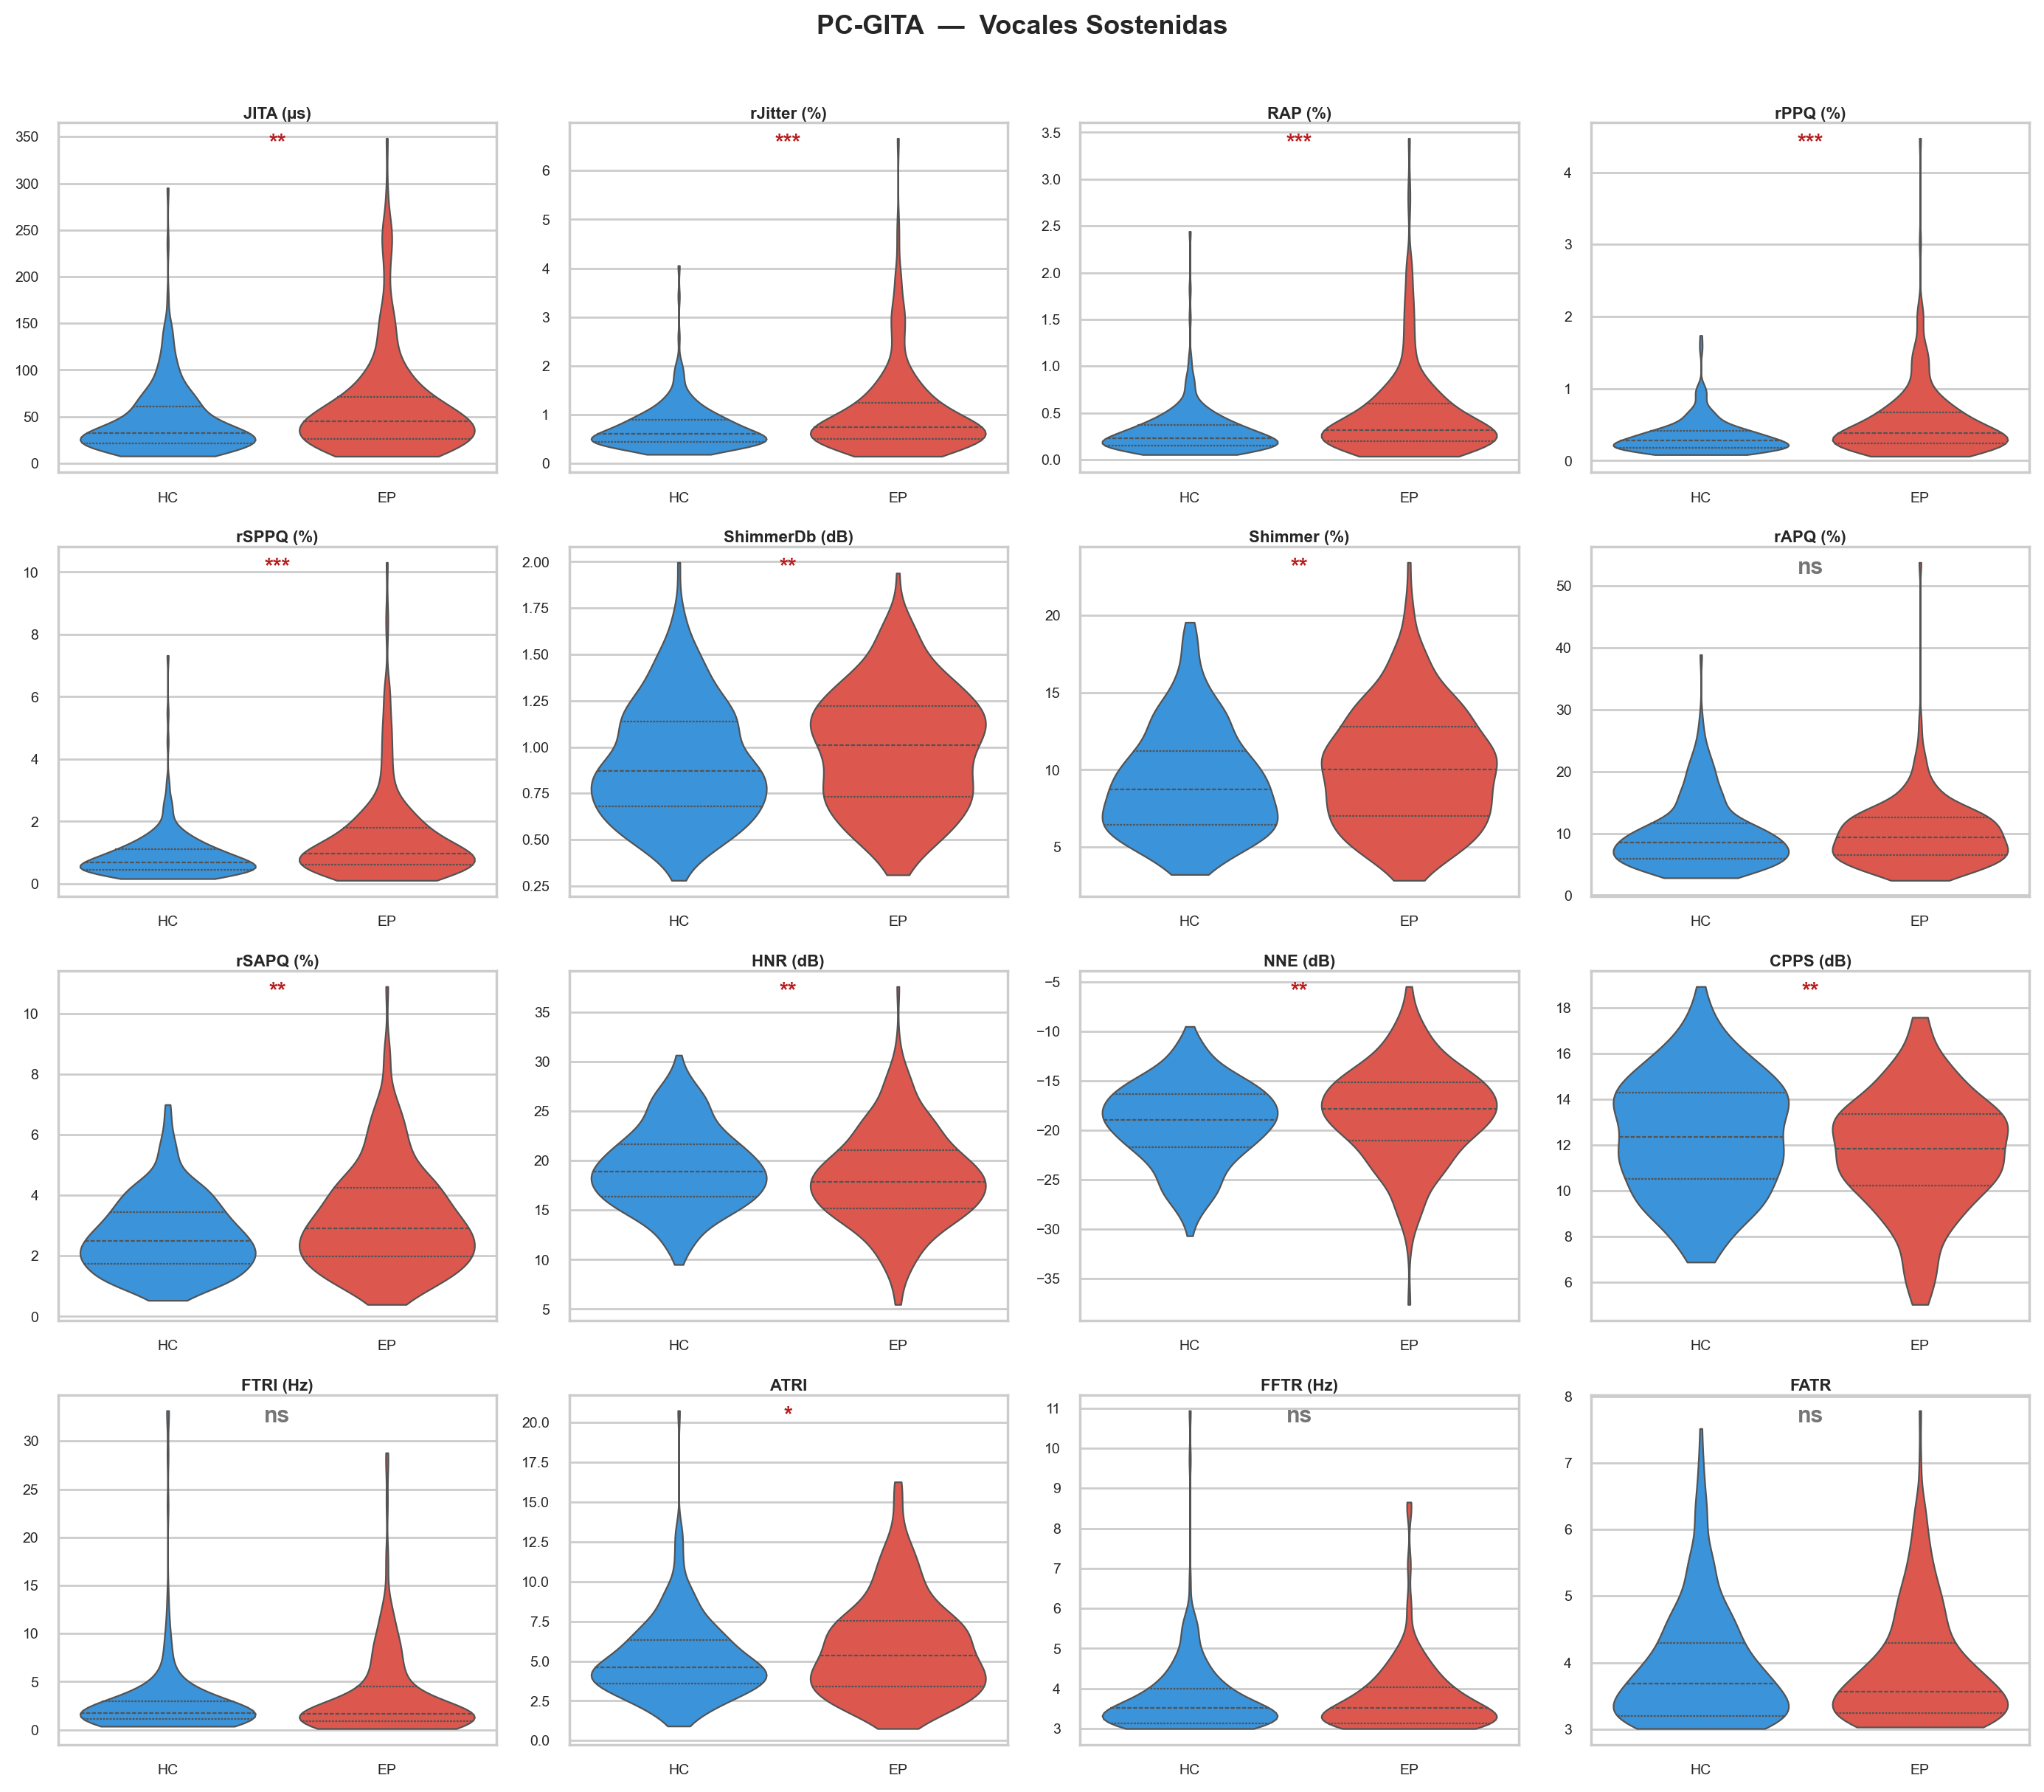
\includegraphics[width=\textwidth, height=0.88\textheight, keepaspectratio]{imagenes/eda/eda_violins_PG_vocal.png}
    \caption{Diagramas de violín — PC-GITA, Vocales Sostenidas.}
    \label{fig:violin_pg_vocal}
\end{figure}

\begin{figure}[p]
    \centering
    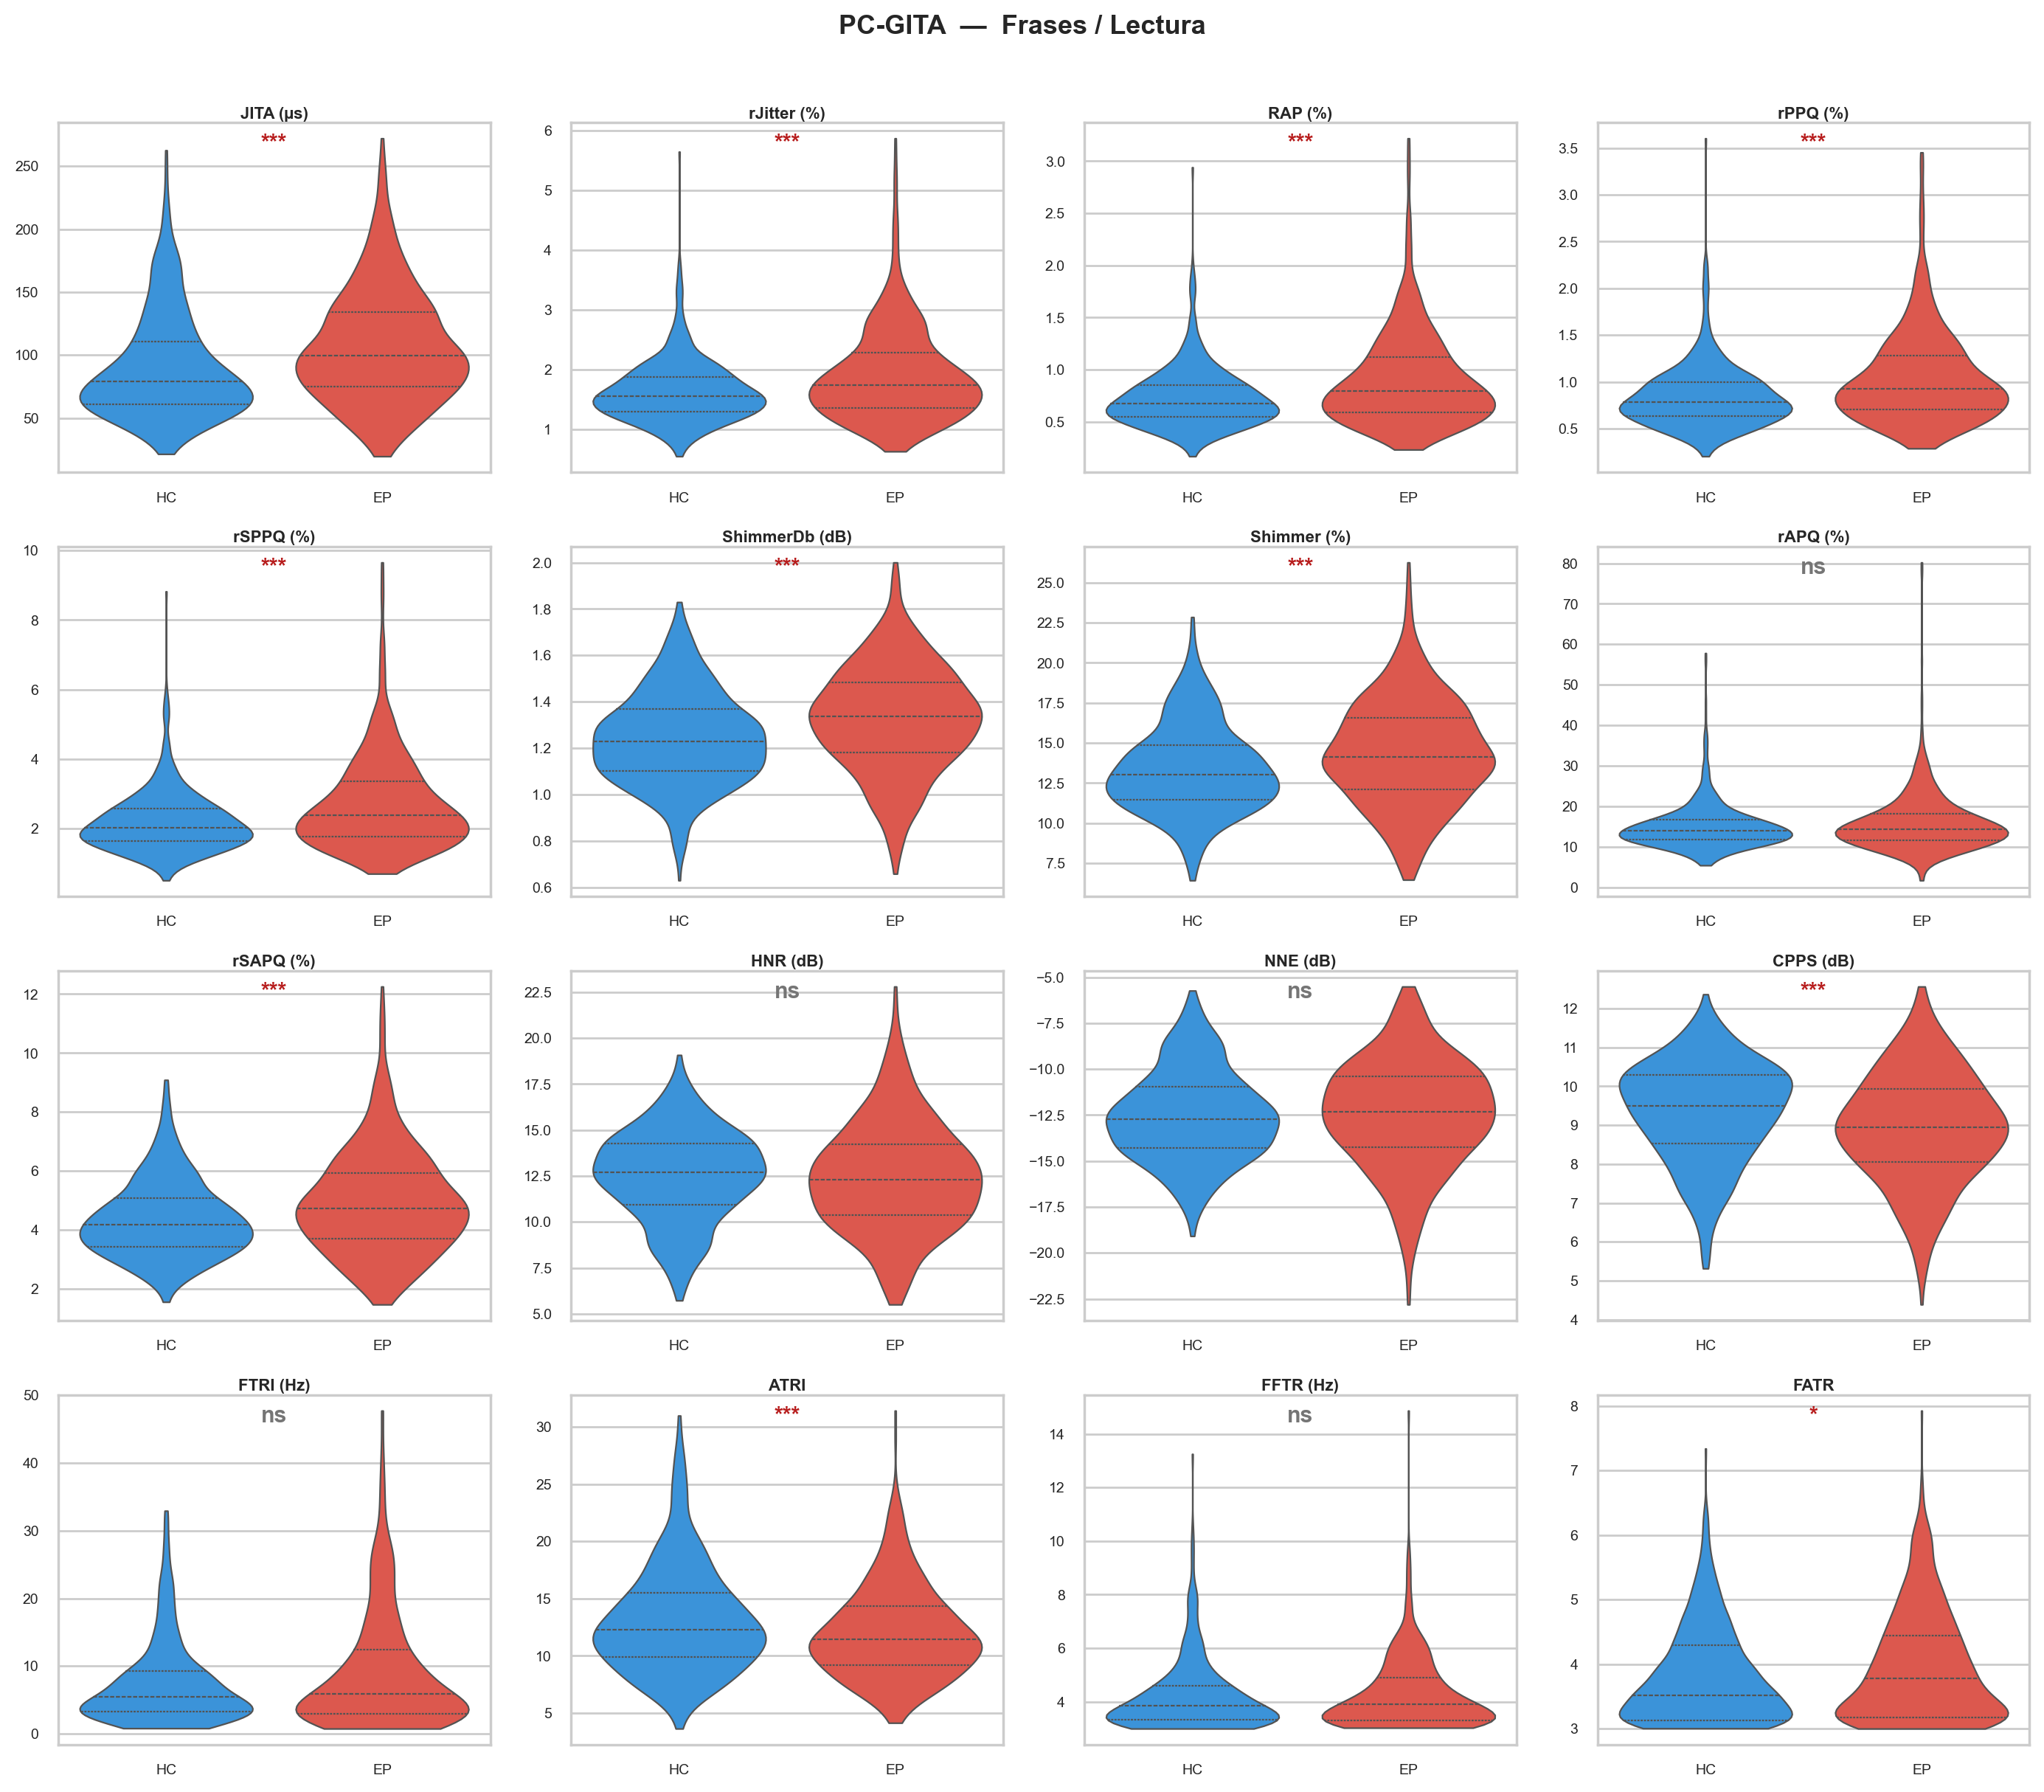
\includegraphics[width=\textwidth, height=0.88\textheight, keepaspectratio]{imagenes/eda/eda_violins_PG_frase.png}
    \caption{Diagramas de violín — PC-GITA, Frases / Lectura. Esta condición presenta las separaciones más pronunciadas entre grupos en todo el conjunto de datos.}
    \label{fig:violin_pg_frase}
\end{figure}

\begin{figure}[p]
    \centering
    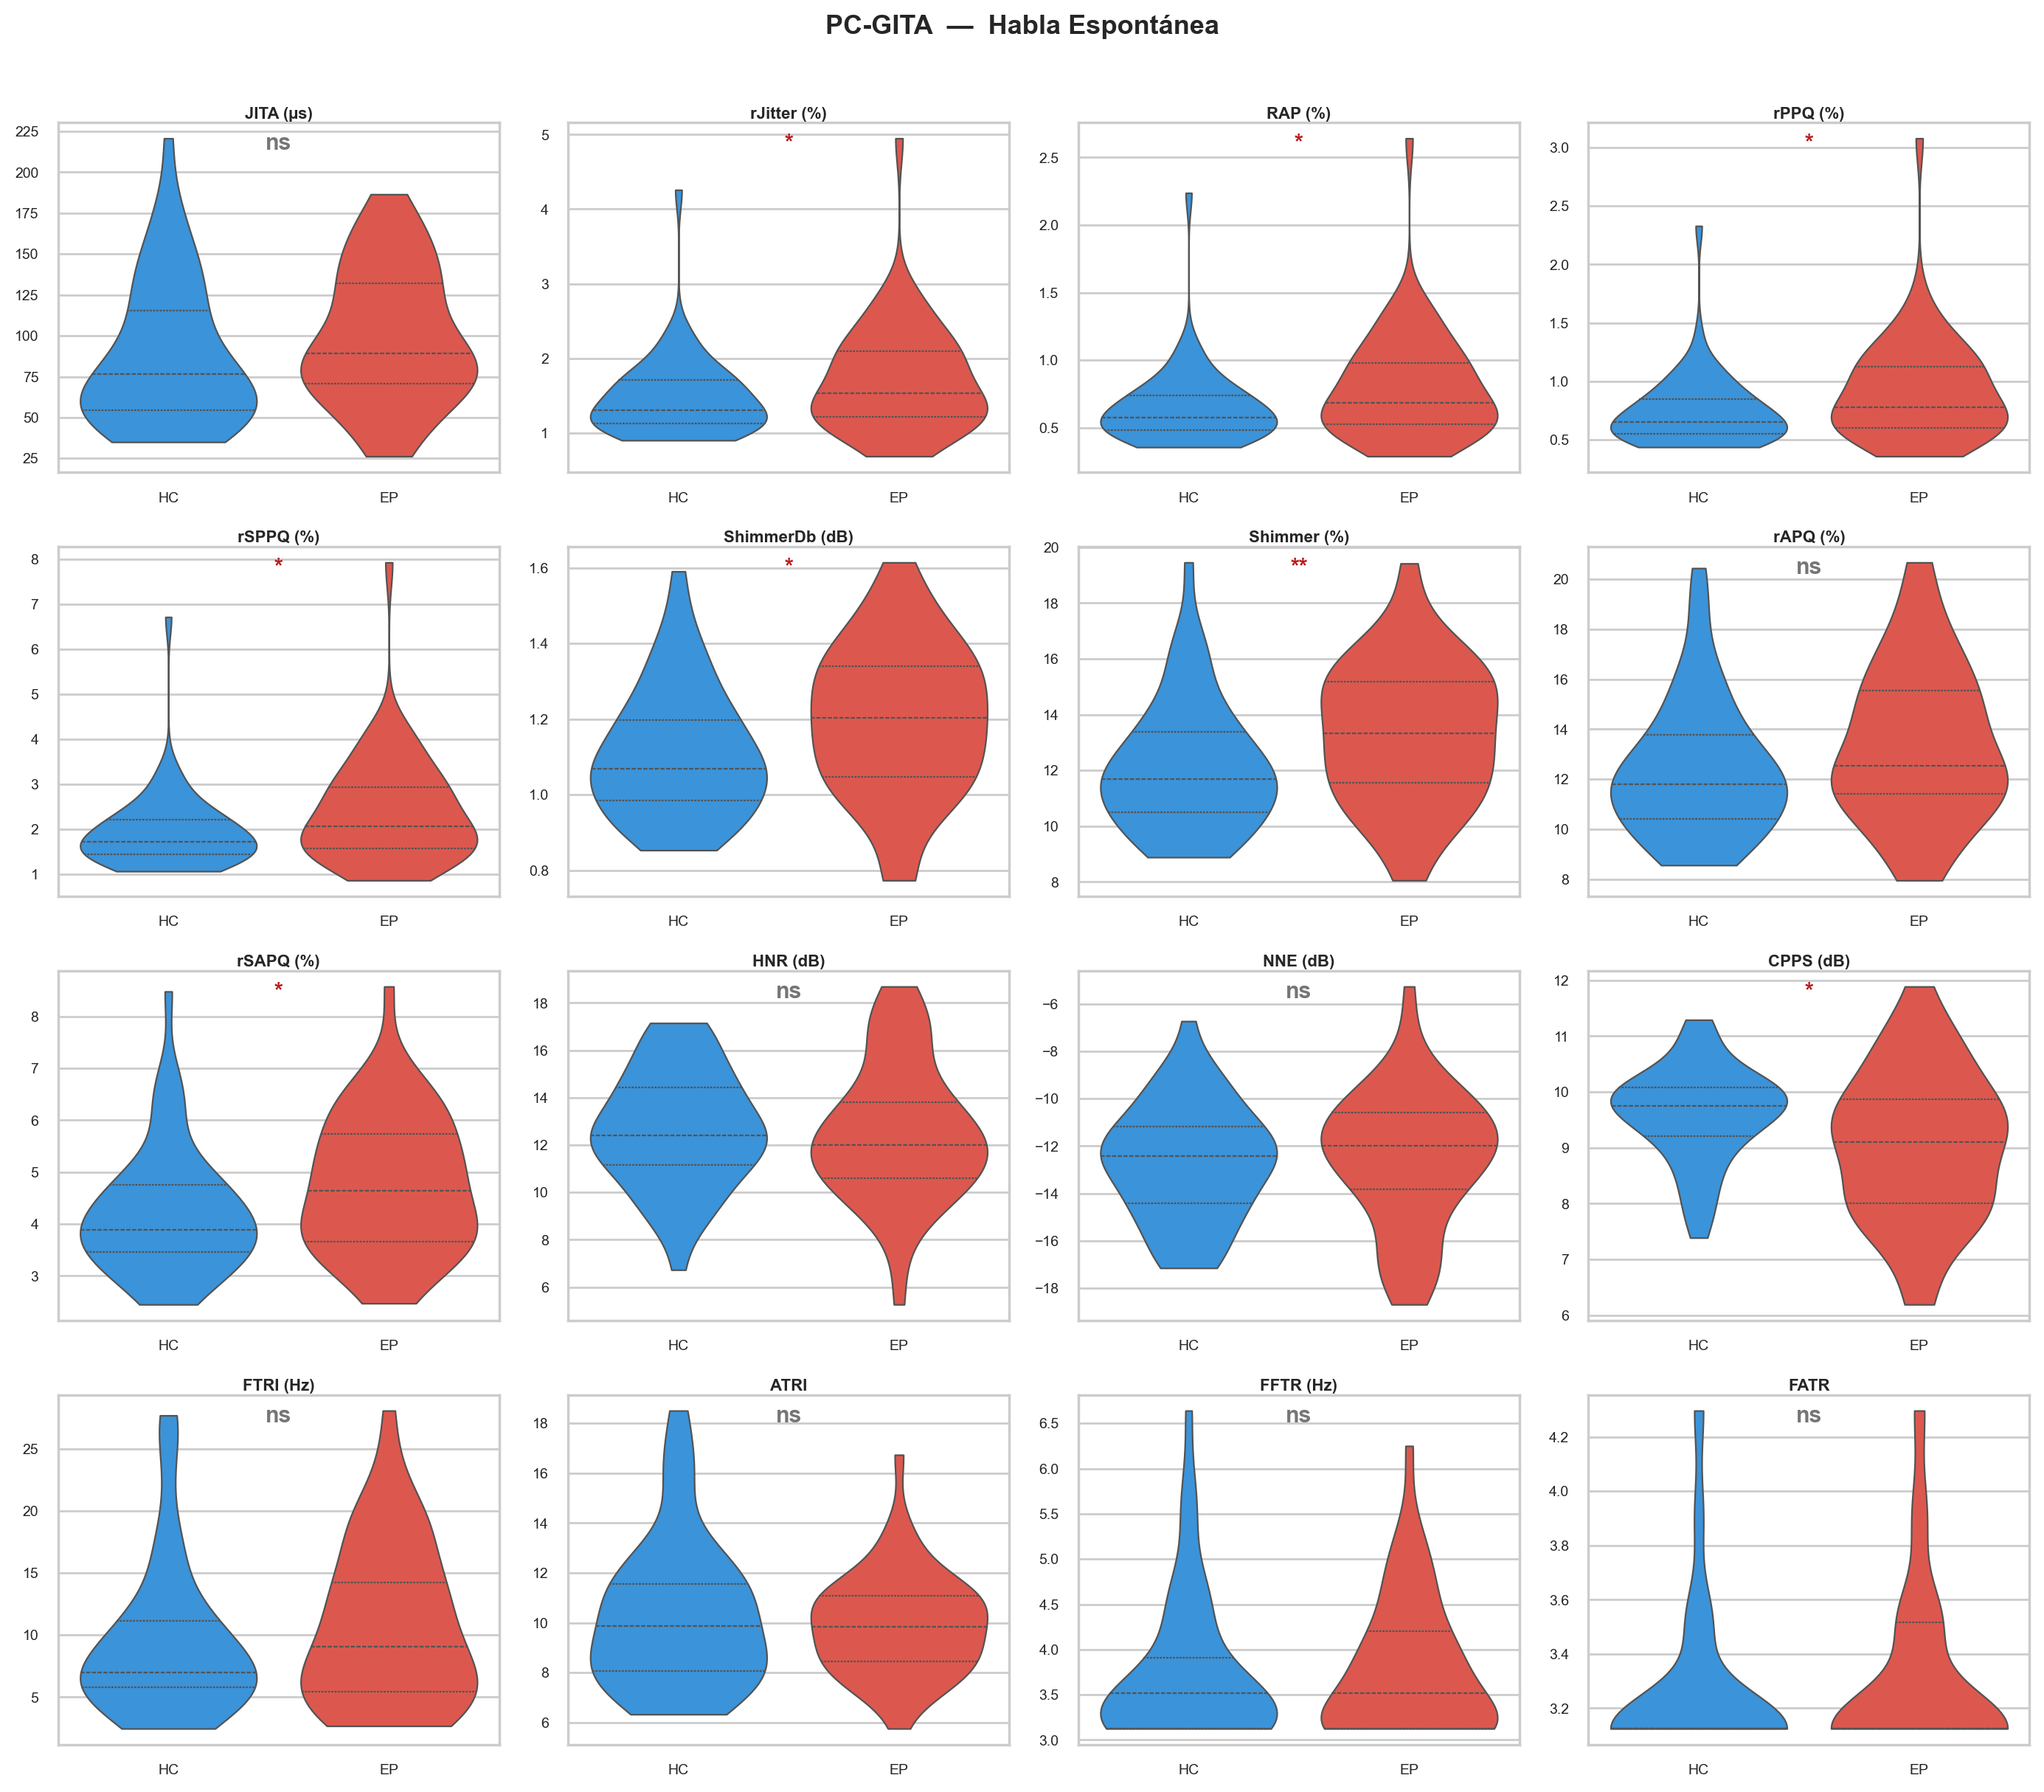
\includegraphics[width=\textwidth, height=0.88\textheight, keepaspectratio]{imagenes/eda/eda_violins_PG_espontanea.png}
    \caption{Diagramas de violín — PC-GITA, Habla Espontánea.}
    \label{fig:violin_pg_esp}
\end{figure}

De la inspección de los diagramas de violín se extraen las siguientes conclusiones por tipo de biomarcador:

\paragraph{Jitter (perturbación de frecuencia).} En \textbf{PC-GITA Vocales} y \textbf{PC-GITA Frases}, todas las variantes de jitter (JITA, rJitter, RAP, rPPQ, rSPPQ) presentan una separación clara: los violines EP están desplazados hacia valores más altos y son más dispersos, reflejando la irregularidad en el control del periodo fundamental. Sorprendentemente, en \textbf{NeuroVoz Vocales} estas mismas métricas no resultan significativas, lo que sugiere diferencias en el protocolo de grabación o en las características de los participantes entre los dos corpus.

\paragraph{Shimmer (perturbación de amplitud).} ShimmerDb y Shimmer son significativos en \textbf{PC-GITA Frases} con una separación muy pronunciada, y en \textbf{NeuroVoz Frases} de forma moderada. En vocales, la separación es menor pero presente, especialmente en PC-GITA. Esto indica que la inestabilidad en la amplitud vocal de los pacientes EP es más manifiesta durante la lectura de frases que en la fonación sostenida.

\paragraph{Armonicidad (HNR, NNE, CPPS).} HNR y NNE destacan en \textbf{NeuroVoz Frases}: los violines HC se concentran en valores altos (voz limpia), mientras que EP se extiende hacia valores menores (mayor componente ruidoso). CPPS presenta significancia en \textbf{PC-GITA Frases} y \textbf{PC-GITA Vocales}, siendo coherente con los resultados del análisis de importancia Random Forest que lo sitúa como el biomarcador más relevante en habla espontánea.

\paragraph{Temblor (ATRI).} ATRI muestra la separación más consistente del conjunto: en \textbf{NeuroVoz Frases} y \textbf{NeuroVoz Vocales} los violines EP son notablemente más amplios y desplazados hacia valores más altos, reflejando el temblor fonatorio de baja frecuencia (3--15\,Hz) característico de la disartria hipocinética parkinsoniana. Es el único biomarcador con separación visible incluso en habla espontánea pese al reducido N.
